\section{Usage}

\begin{frame}{Outline}
    \tableofcontents [current]
\end{frame}

\begin{frame} {Code sample}
%	\begin{verbatim}
%	#define LED_PIN 13
%	 
%	void setup () {
%	 pinMode (LED_PIN, OUTPUT); // enable pin 13 for digital output
%	}
%	 
%	void loop () {
%	 digitalWrite (LED_PIN, HIGH); // turn on the LED
%	 delay (1000); // wait one second (1000 milliseconds)
%	 digitalWrite (LED_PIN, LOW); // turn off the LED
%	 delay (1000); // wait one second
%	}
%	\end{verbatim}
\end {frame}

\begin{frame} {Documentation}
	On the arduino.cc website
	\begin{itemize}
		\item Simple, Readable, Relevant 
		\item open access (and edit) wiki, 
		\item regular updates
	\end{itemize}
\end{frame}

\begin {frame} {Documentation}
	For all pages about a subject, there are
	\begin{itemize}
		\item hardware scheme
		\item code samples, with relevant comments, Creative Common licence
	\end{itemize}
\end {frame}

\begin {frame} {Examples}
	\begin {center}
		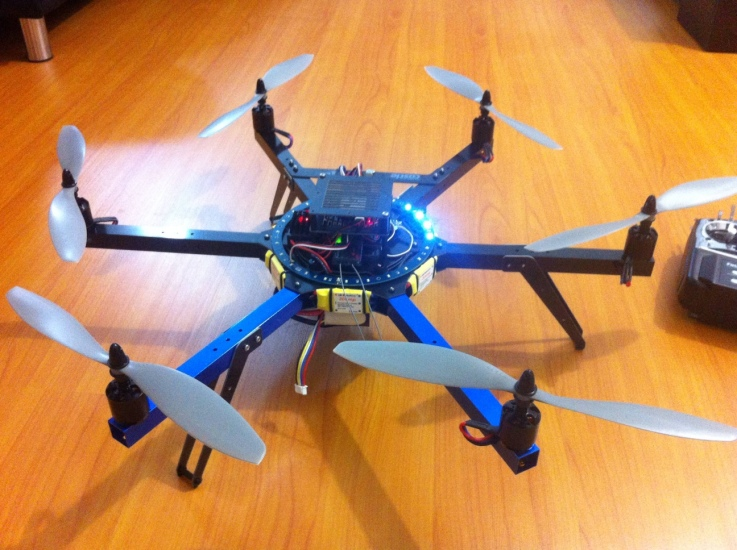
\includegraphics [width=.7\textwidth,keepaspectratio] {img/drone}
	\end {center}
\end {frame}

\begin {frame} {Examples}
	\begin {center}
		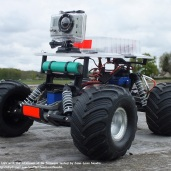
\includegraphics [width=.5\textwidth,keepaspectratio] {img/rover}
	\end {center}
\end {frame}
